\chapter{问题分析与研究框架}
\label{cha:problem_framework}

\section{本章引论}

面向文本的情感识别和相关研究多种多样,如前一章中提到的面向评论的五星评分预测、面向微博的正负中性情感识别、面向评论的五级反讽强度识别等。虽然这些课题关注的文本特征不同,需要区分的类别不同,采用的数据处理技术和算法也因此有所不同,但它们在本质上有相同之处,其研究方法大同小异。

本章的内容安排如下。在章节~\ref{sec:global_problem_analysis}中,我们将首先分析情感识别的分类问题所涉及的要素,并给出统一的形式化表示。基于该形式化表示,在章节~\ref{sec:global_framework}中,我们会提出一个面向文本的情感识别研究框架,说明每个步骤中需要实现的功能和目的,在后续章节中,我们将基于此研究框架开展工作。在章节~\ref{sec:technology}中,我们会根据研究框架中需要实现的各种功能,介绍其相对应的技术。

\section{问题分析}
\label{sec:global_problem_analysis}

本节将对面向文本的情感识别所涉及的各项要素作出分析,并给出统一的形式化表示,以描述这些要素之间的关系。

在情感识别的分类问题中,需要把情感区分为有限个不同的类别,这些类别组成情感集合$C$。如Tang等人\cite{tang2015learning}的情感极性识别研究,$C$对应五个级别的情感。在刘丹丹等人\cite{刘丹丹2015基于}的微博情感分类研究中,$C$对应情感类别为喜好、安乐、惊奇、厌恶、悲哀、愤恨、恐惧。另外在反讽识别问题中也同理,在邓钊等人\cite{2015面向微博的中文反语识别研究}的中文反语识别研究中,$C$则对应包含反讽和不包含反讽这两个类别。

而在面向文本的情感识别问题中,必然有文本内容$T$,它由情感持有者$S$发表,是他表达个人想法和情感的载体。在一些场景下还会有上下文$B$,对应和$T$相关的内容,有助于了解$T$表达的意思。譬如在研究讨论区上帖子的情感类别时,$T$对应帖子的文本内容,$S$则是帖子的发布者。而帖子所在讨论区的类型有助于定位帖子对应的主题,发布者的发布历史可能隐藏发布者的一些态度倾向,帖子下的评论从侧表反映主帖的内容,这些都可以作为上下文$B$。又以Zahiri等人\cite{Zahiri2017Emotion}对电视剧台词的情感识别研究为例,$T$对应电视剧中的台词,$S$为说台词的对应角色,其他角色的台词可以作为上下文$B$。

那么对于任意一段文本$t \in T$,在给定上下文$b \in B$的情况下,情感识别假设$t$表达的情感必然对应某种情感类别$c \in C$。我们的目标是找出一个映射关系$f$,使得 $c=f(t, b)$。

\begin{figure}[H]
  \centering
  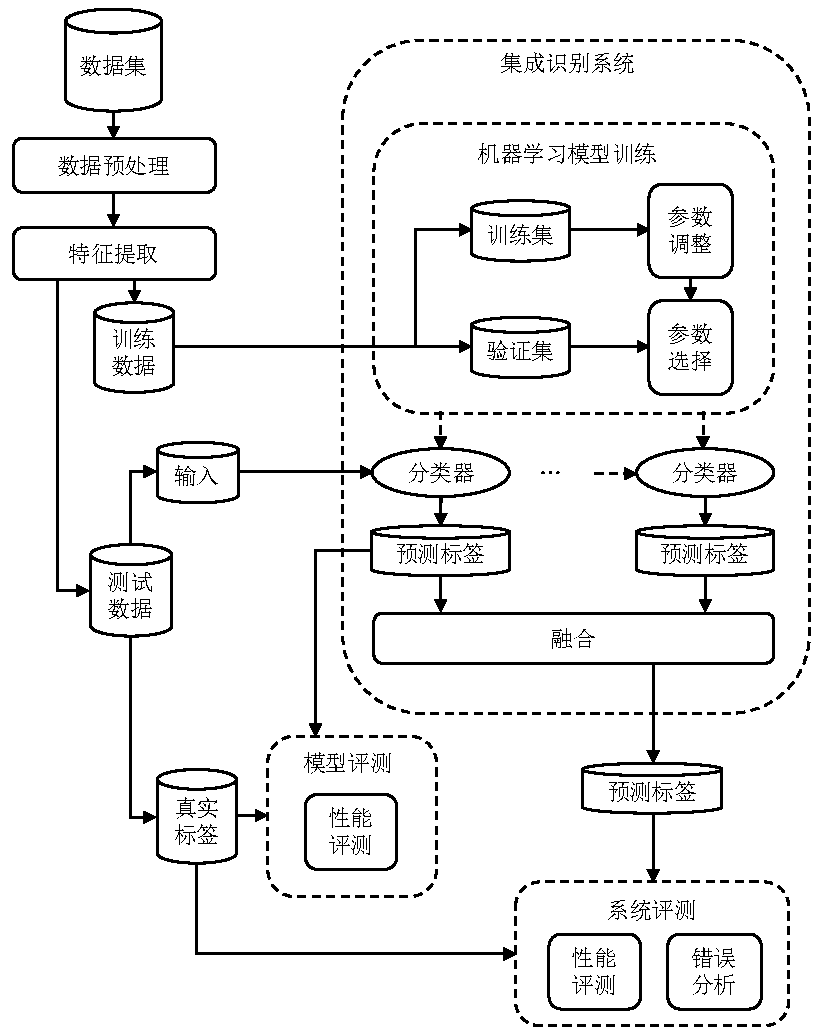
\includegraphics[width=0.8\textwidth]{img/framework_v2.pdf}
  \caption{情感识别的研究框架}
  \label{fig:framework}
\end{figure}

\section{研究框架}
\label{sec:global_framework}

在本小节,我们将给出一个情感识别分类问题的研究框架,并给出其中每一步需要完成的任务和目的。图~\ref{fig:framework}显示本文面向情感识别的研究框架。

如图所示,整个框架的输入是实验的数据集,数据集的每个样本包含三个元素,分别是目标的文本、其对应的上下文以及原文本的情感类别标签,参考章节~\ref{sec:global_problem_analysis}的形式化表示,每个样本可以表示为 $<t, b, c> \in T \times B \times C$。其中目标文本$t$和上下文$b$都需要首先进行预处理和特征提取以得出其量化后的特征,作为识别系统中各个模型的输入。然后整个数据集会被分成训练数据和测试数据,分别用于识别系统的开发和评测。

对于一个多分类问题,我们可以把它分解成多个子分类问题的叠加。如面向正负中性情感的三分类问题,一些研究工作会首先判断文本的情感属于主观还是客观(中性),再将带主观情感的样本区分为正性和负性情感,即原本的三分类问题被拆解成主观和客观二分类以及正负性情感二分类两个问题的叠加。因此,我们再把接下来的研究工作分成两个阶段。

在第一阶段,首先分别研究原问题所涉及的各个子问题,分析不同算法在各个子问题上的性能。这一阶段中对每个子问题的研究工作可以分成以下几步:

\begin{enumerate}

\item 基于不同模型得出分类器。而对于机器学习方法,标准流程是首先把训练数据分成训练集和验证集,利用训练集对模型的参数进行多轮的调整,每一轮分别得出一组模型的参数,然后评估每一组参数在验证集上的性能,最后取其中性能最好的一组参数作为分类器的参数。

\item 对测试集的样本进行预测。基于各个模型训练得出分类器后,分别预测测试集上各个样本所属的类别,得出预测标签。

\item 性能评测。对比预测标签和真实标签,计算各项评价指标。透过比较不同模型在各项指标上的差异,一方面可以了解各模型对该问题的建模能力,另一方面结合各模型的结构,从侧面了解语料背后的数学模型。

\end{enumerate}

在第二阶段,基于各个子分类问题组成一个集成识别系统,并分析其性能和特性。研究工作包括以下几步:

\begin{enumerate}

\item 为各个子分类问题训练分类器。基于第一阶段中对各个模型性能的分析结果,为各个子分类问题选定合适的模型,并训练一组分类器。

\item 对测试集的样本进行预测。对于测试集上的每一个样本,按照一定顺序由对应的分类器组回答各个子分类问题,以此得出最终的预测标签,同时保留其中的中间结果。

\item 性能评测。对比预测标签和真实标签,计算各项评价指标。另外还会观察系统的中间结果,了解每个子分类问题的设置对整个系统的识别能力的影响。

\item 错误分析。观察在测试集上样本被系统误判的原因,观察各个类别之间是否有明显的相互混淆的情况,透过深入分析指出系统的不足以及改进的方向。

\end{enumerate}

在后续章节中的每组实验,我们都将基于此研究框架进行我们的工作。

\section{相关技术}
\label{sec:technology}

在本节中,我们将对研究框架中的文本预处理、特征提取、机器学习方法、集成学习方法进行介绍,分别说明它们的目的、具体技术和原理。对于在后续实验用中使用到的技术,我们会给出相对充分的说明,同时也会为相关的技术给出概要的描述,以便读者在本论文未深入探索的方向进行拓展性的工作。

\subsection{文本预处理}
\label{ssec:text_preprocess}

文本预处理是所有面向文本的研究的第一步,其目的是为特征提取做好准备。好的预处理策略可以在尽可能不掉失重要信息的情况下对样本数据进行简化,使样本之间重复的模式更容易被识别,降低算法对数据进行拟合的难度。错误的预处理策略会丢失具有区分能力的信息,甚至产生具有误导性的样本。对于不同的语言,由于存在语用和语法等方面的不同,预处理的方法也会各异。本小节将针对社交媒体上的英语文本介绍几种预处理技术。

\subsubsection{分词}
\label{sssec:tokenization}

为了从文本提取词级别的特征,我们需要首先将句子分解成多个词的序列。

虽然对于英语及大部分西方语言,空格隔开的字符必然属于不同的单词,但对于不以空格分隔的语言(如中文),分词的作用尤其重要。在某些情况下,分词的结果会影响对句子的理解,如将“乒乓球拍卖完了”分解成“乒乓球拍-卖-完-了”或“乒乓球-拍卖-完-了”,对主体应该是“乒乓球拍”还是“乒乓球”,动词应该是“卖”还是“拍卖”,仅凭字面意思无法确定发言者想表达的意思。特别地社交媒体平台上,新词不断的出现,要正确进行分词就有其独特的难点。而分词并不只针对语言中的单词,还针对由标点符号和其他特别字符组成的有一定语义和情感的字符组合,如现今社交媒体上普遍用多个字符拼接成颜文字,其中最常见的有微笑的表情“:)”和伤心的表情“:(”,但如果在分词过程中把前者分割成“:”和“)”就会丢失其带有正向情感的信息,这在短文本的情感识别中非常关键。

虽然利用空格和标点符号在大部分情况下可以完成对英语句子的分词,但在一些情况下,标点符号作用为词组的一部分而不是分隔符,另外在社交媒体上也会有空格被省略的情况,以下是英语中一些需要额外处理的情况\cite{jackson2007natural}\cite{mitkov2004oxford}。一是带句号的缩写,如“U.S.”、“.com”,句号应该作为词的一部分,如果按句号切割“U.S.”将失去其原本的语义。二是具有一定格式的带标点符号的词组,如电子邮箱地址(如example@email.com)、时间(如 Jan 6th、06/01/19)、电话号码(如(123)456-7890)、网页地址(如www.example.com)等,这些内容在大部分情况下可以被视为一个个体,我们更关注这个个体对应什么类型的事物,而不是其细节,譬如将一个句子中电话号码的具体数字替换掉并不会改变其情感的表达,但识别出一个字符串对应的事情类型,并在清楚它对情感识别没有关联的情况下对其忽略是有意义的。第三种情况是附属词,如“'t”对应“not”,只有正确识别“'”的作用才能识别出否定的意思,否则句子的意思将完全相反。值得注意的是,对社交媒体平台上的文本,除了以上在正规英语中会出现的情况,还会出现其他特殊情况,如“Y!E!S!”和“N!O!”。这需要对数据首先进行人工观察找出特殊的模式,再对语料库进行统计判断其出现频率,若出现频率较高则新增处理规则将对应模式做转换(如将“Y!E!S!”替换成“YES!!!”)或对问题无关的模式忽略(如国外某微博平台以“RE:”开头表示回复,并不包含任何情感,可以忽略)。

\subsubsection{拼写修正}

在处理较正式的文件时,一般可以默认其文本满足语言规范,词汇基本都是正确的拼写。不过在社交媒体上,拼写不符合规范的情况则非常普遍,这些情况可以分成三大类。

第一类是非刻意的拼意错误,由于社交媒体上的文本普遍是非正式的,用户不会刻意去保证文本的语言正确性,他们更关注于表达自己的想法和情感。拼写修正技术一般基于统计的方法,对于一个不存在的词汇,尝试对其拼写进行有限次编辑,再评估编辑后的词在其上下文中出现的概率,最后选出可能性最高的一个词作替换。拼写修正技术已相当成熟地被应用于搜索引擎和手机键盘等应用中,读者可参考相关研究\cite{ahmed2009revised}\cite{nejja2015context}了解其细节。

第二种情况是网络上常用的代替用词,如以“thx”、“tnx”代替“thanks”,以“k”代替“ok”,以“cant”代替“can't”。虽然这些用法没有被认可为标准用法,但由于方便而在网络上被广泛传播,成为网民们都能理解和接受的用法。对此的处理方法有两种,一是人工建立映射表,把代替用词映射到标准的英语词汇,优点在于可以直接引用标准词汇的语义信息,但缺点是需要人工参与,特别是在网络上新用词不断出现的情况下需要持续的更新。另一种是不做处理,利用机器学习方法从大型语料库中自动学习出它的语义,优点在于省去了人工的部分,缺点在于新词的出现很稀疏,严重依赖于语料的收集。

第三种情况是语气加强,如“yeeeees”、“AMAZING”,但对于这一类情况,处理的重点不只在于转换成标准用词,而是根据具体的研究问题判断是否要识别这种语气的加强作为提示信息,譬如在情感识别中,语气加强一般提示了此处表达的情感较强烈。Baziotis等人\cite{baziotis2017semeval2}的做法是在单词前后添加标签示意,如“yeeeees”替换成“yes <enlongated>”,“AMAZING”替换成“amazing <allcaps>”。

\subsubsection{规范化}

在章节\ref{sssec:tokenization}中曾提及在一些特定的应用场景下,电子邮箱地址和日期等内容的细节其实对我们的研究任务并不起作用,因此我们可以用一个特定的单词代替相同类型的内容。如Kouloumpis等人\cite{kouloumpis2011twitter}在处理微博文本时将不同的网页地址和“@用户名”分别用特定的字符串代替。更进一步地,Baziotis等人\cite{baziotis2017semeval2}在研究情感识别时,将表达同一种情感的不同表情符替换成对应的情感标签,如“:)))”替换成“<happy>”,“:-D”替换成“<laugh>”。但需要注意替换的内容是否会导致信息掉失,如Joshi等人\cite{joshi2015harnessing}在针对反讽识别的研究中指出一些反讽透过具体数字的对比来表达,在这种情况下将具体数字统一替换成表示数字的标签可能会导致预处理后的样本失去原本的反讽属性。

\subsection{特征提取}
\label{ssec:feature_extraction}

数据经过预处理后,我们需要从获得的字符串或字符串序列中提取任务相关的特征,并进行量化方可作为分类器的数学模型的输入。本小节将介绍几种主流的文本特征提取技术。

\subsubsection{词嵌入}
\label{sssec:embedding}

词嵌入即捕足词的语义、语法、情感等信息并将其以向量表示。其中词对应预处理中分词得到的词,或对于字符级别的模型,“词”可以对应单个字符\cite{baziotis2018ntua}。主流的词嵌入算法分成两大类:基于人工神经网络的方法和基于矩阵分解的方法。

基于人工神经网络的方法假设句子中词之间存在某种上下文关系,并以神经网络建模学习,其中最具代表性的是CBOW和Skip-gram两种算法。CBOW的建模原理是句子中的一个“词”可以由它在句子中的前后有限个“词”决定,Skip-gram的建模原理则是句子中的“词”可以推测出它在句子中的前后有限个“词”。这两种算法都在自然语言处理中常用的词嵌入学习工具Word2vec\cite{mikolov2013efficient}中提供,又由于训练优质的词嵌入模型(指一组词到词向量的映射)需要收集大量的数据和耗费相当的时间,一些利用Word2vec训练好的词嵌入模型会作为公开的资源供其他研究员使用。其中较常用的是谷歌提供的模型\footnote{https://code.google.com/archive/p/word2vec/},利用谷歌新闻作为语料训练出复盖约三百万个词的三百维向量集合。然而词向量所包含的信息和语料库紧密相关,所以也有一些研究会按照自己课题的特性自行收集相应的语料来训练词向量。如Baziotis等人\cite{baziotis2017semeval2}利用微博平台Twitter上收集的数据训练词向量模型并应用于面向微博的反讽识别,其词向量模型也被公开供其他研究者使用\footnote{https://github.com/cbaziotis/ntua-slp-semeval2018}。

\begin{figure}[H]
  \centering
  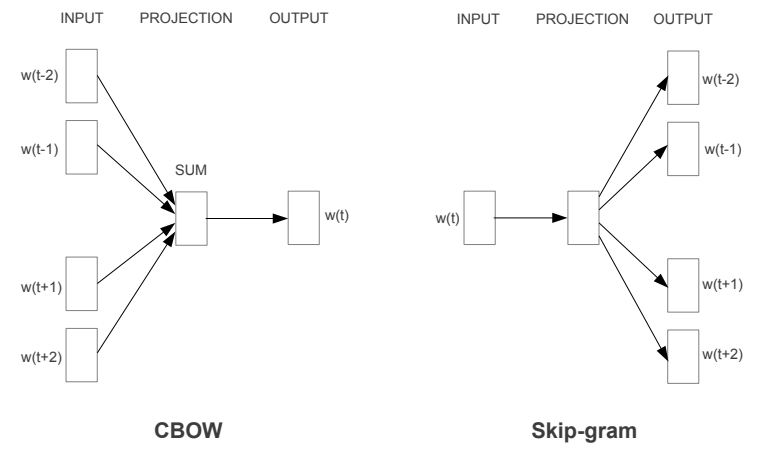
\includegraphics[width=0.8\textwidth]{img/word2vec.png}
  \caption{Word2vec提供的两个算法的模型,引自\cite{mikolov2013efficient}}
  \label{fig:word2vec}
\end{figure}

基于矩阵分解的方法假设一个表示词和词或词和文档之间关系的矩阵可以表示为由词向量组成的矩阵和其他矩阵的相乘,因此对该关系矩阵以对应方式进行矩阵分解即可以得到词向量。具代表性的方法是隐藏语义分析方法(Latent semantic analysis,LSA)\cite{deerwester1990indexing},以词在各个文档中出现的频率得出词-文档矩阵,并假设其文档可以表示为词-词概念、词概念-文档概念、文档概念-文档三个矩阵相乘,利用奇异值分解(Singular Value Decomposition,SVD)得到词-词概念矩阵,取每一行作为对应词的词向量。另外还有Pennington等人\cite{pennington2014glove}提出的GloVe算法,该算法根据不同词在语料中出现在各自上下文窗口中的频率得出词和词之间的关系矩阵,再分解成两个词-词概念矩阵的相乘。其研究结果显示在部分自然语言处理任务中,采用GloVe较Word2vec及另外几种词嵌入技术得出的词向量能达到更好的效果。他们同样公开了多个利用不同语料库训练好的词向量模型供其他研究者使用\footnote{https://nlp.stanford.edu/projects/glove/}。

\subsubsection{词汇特征} % Lexical Feature 

词汇特征表示文本中一元或多元语法的分布情况,不考虑词的具体意思。譬如常用的词袋模型(Bag of words, BOW),其将一段文本映射到一个固定长度的向量,向量上每一维对应一个一元或多元语法的某种属性,譬如它是否在文本中出现(即独热编码),或它在文本中出现的频率,或其词频-逆文档频度(Term Frequency - Inverse Document Frequency,TF-IDF)。或更简地以单词数量或字符数量作为一维的特征。

\subsubsection{句法特征} % Syntactic features 

句法特征表示文本中各个词在句子的语法作用。常见做法是先对文本进行词性(Part-of-speech,POS)标注和依赖树分析,再基于标注提取特征,如形容词的数量、副词的数量,或以标注代替单词后采用词袋模型得出固定长度的特征向量。一些研究会针对性地手工设计句法特征,这要求研究者对语法有所了解并挖掘它对研究问题是否存在关联性,相对地这种特征的解释性更强。

\subsubsection{语义特征} % Semantic features

语义特征基于文本的字面意思,表示文本表达的内容或其中的个别属性‌(如主题分布),这更接近于人们透过理解句子内容来进行识别。常见技术譬如基于文本中各个词所对应词向量计算句子的表示向量,或利用词向量计算句子中各单词和情感词的相似度来间接评估词的情感极性,或利用聚类算法对语料库的单词进行聚类来获得单词的隐藏语义类别,再计算句子中各类别单词的分布。

\subsection{机器学习方法}
\label{ssec:model}

本小节将给出搭建情感识别系统相关的机器学习方法。目前用于情感识别的主流算法可以分成两大类:传统机器学习和人工神经网络。我们会分别对这两类算法中具代表性的例子给出介绍。

\subsubsection{传统机器学习}
\label{sssec:traditional_ml}

支持向量机(Support Vector Machine, SVM)\cite{cortes1995support} 由Cortes和Vapnik在1995年提出,是目前最常用的传统机器学习算法之一。在对二分类问题的建模过程中,每个训练样本被映射到一个空间中的一个点,而支持向量机尝试找出一个边缘把空间分成两个子空间(如以直线分割二维空间,以平面分割三维空间),每一个子空间对应一个类,使得训练样本尽可能落在对应类别的子空间中。对于多分类问题,主流做法是把原问题拆解成多个二分类问题。后随着核函数的引入,将支持向量机拓展成非线性的数学模型,大大加强了其建模能力。除了分类问题,支持向量机同样可以应用于回归问题,Drucker等人\cite{drucker1997support}则提出了支持向量机的回归模型。支持向量机最大的限制之一是只接受固定长度的向量作为输入,要求从输入数据提取出固定长度的特征向量,换言之基于支持向量机的识别系统非常依赖对特征的提取。

\begin{figure}[H]
  \vspace{-5mm}
  \centering
  \captionsetup{width=.8\linewidth}
  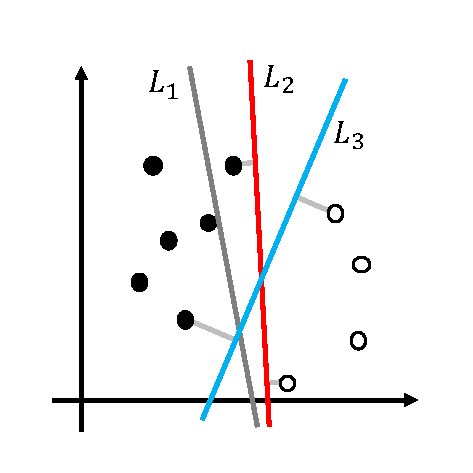
\includegraphics[width=0.35\textwidth]{img/svm.pdf}
  \caption{支持向量机在处理二类问题的示情感。其中黑点和白点分别对应两个类别的样本,$L_1$不能对两类样本作区分,$L_2$和$L_3$均成功区分两个类别的样本,但$L_3$和两个类别样本的距离更大,为更优解}
  \label{fig:svm}
\end{figure}

决策树(Decision Tree)是另一种常见的机器学习方法。对于分类问题,决策树基于训练数据建立一个树状模型,其中每个非子叶结点对应一个决策,叶子结点对应要识别的类别。在识别阶段,识别过程从根结点开始,经过每个非叶子结点根据输入数据得出决策结果,不同的决策结果会对应下一级的一个结点,如此不断前进直到到达叶子结点,以其对应类别作为分类结果。和支持向量机一样,决策树的输入为固定长度的向量,要求对应的特征提取。现今的研究更多地会使用由多个决策树组成的随机森林(Random Forest)而非单个决策树作为分类器,随机森林属于集成学习一类,将在后续章节\ref{ssec:intro_ensemble_learning}中介绍。

\subsubsection{人工神经网络}

人工神经网络源自仿生学,以数学模型模拟生物神经网络的响应过程和学习过程。Rosenblatt提出的感知器\cite{rosenblatt1958perceptron}是最早的人工神经网络,也是现在人工神经网络的基本单元(又称为神经元)。Rumelhart等人\cite{rumelhart1985learning}在后来提出了一种多层前馈神经网络,BP网络,由多层的感知器和激励函数反复堆叠而成。更重要的是他们提出了它的学习算法,反向传播算法(Back-propagation,BP),当网络的输出结果和预期结果不同,透过构造损失函数计算偏差,再根据损失函数和偏差计算出神经元权重的梯度,其对应了使误差扩大的权重方向,以其反方向作为权重修改的依据。同时将该层输入的修改量作为前一层输出的偏差,逐层重复修改权重,整个过程重复迭代直到误差满足一定条件时学习过程结束。反向传播算法是目前人工神经网络模型训练中的核心算法,但随着网络层数增加,梯度以指数级别增大或缩小,会导致梯度大小过大或接近于零的情况,即梯度爆炸和梯度消失。直到Hinton等人\cite{hinton2006fast}提出深度信念网络和无监督逐层训练的策略,其核心思想是在每一轮训练只调整网络中一层的权重,透过固定前一层的输出作为本层的输入,避开了多次传播带来梯度的指数级变化。如此网络逐层经过调整后,再对整个网络进行权重调重,理论上此时的梯度较小,避免了梯度爆炸的出现。这使得现在复杂人工神经网络的学习成为了可能,深度学习正式进入高速发展的阶段。接下来我们将对主流的人工神经网络单元作出介绍。

\begin{figure}[H]
  \centering
  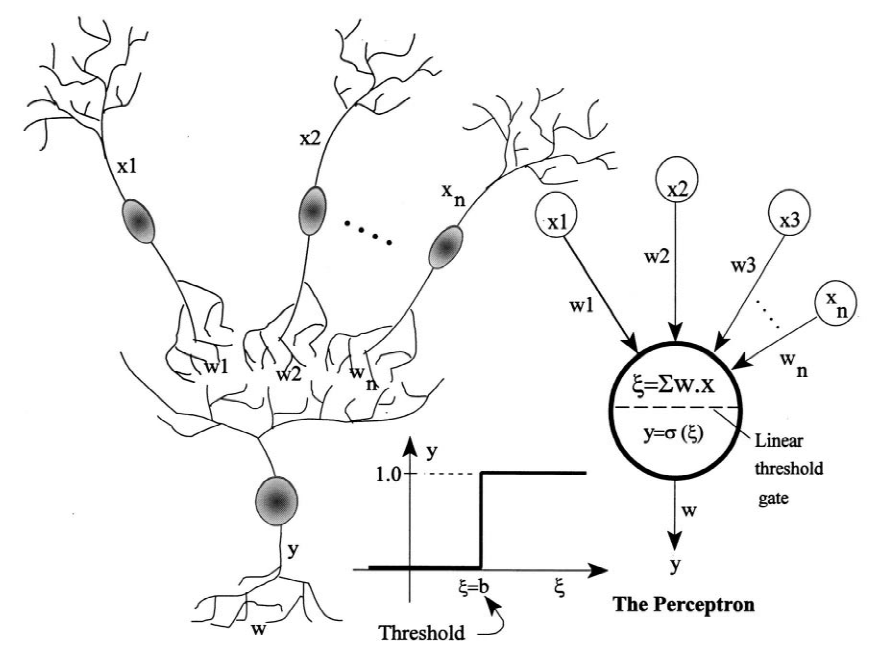
\includegraphics[width=0.7\textwidth]{img/perceptron.png}
  \caption{生物的神经元与感知器的模型示意图,引自\cite{basheer2000artificial}}
  \label{fig:perceptron}
\end{figure}

\begin{figure}[h]
  \centering%
  \subcaptionbox{Lecun等人\cite{lecun1989backpropagation}的反向传播网络
  \label{fig:lecun1989backpropagation}}
    {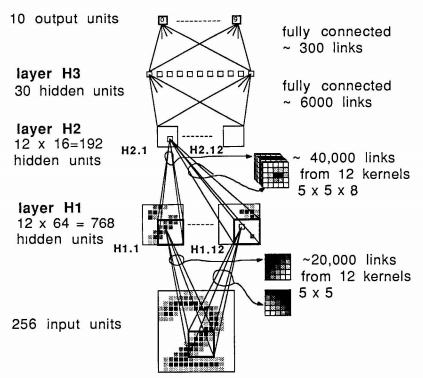
\includegraphics[width=0.42\textwidth]{img/lecun1989backpropagation.png}}%
  \hspace{4em}%
  \subcaptionbox{Waibel等人\cite{waibel1995phoneme}的时延神经网络\label{fig:waibel1995phoneme}}
      {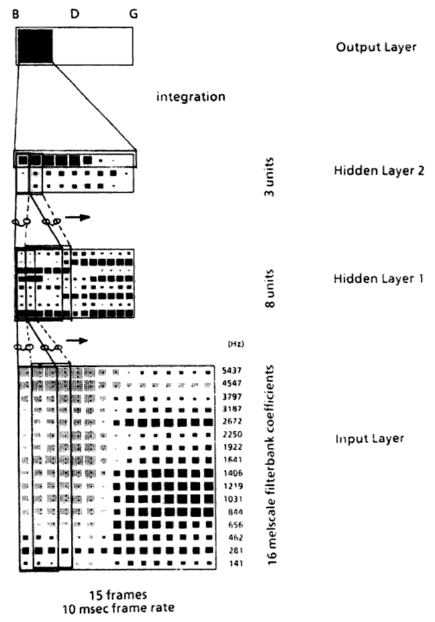
\includegraphics[width=0.42\textwidth]{img/waibel1995phoneme.png}}
  \caption{卷积神经网络模型}
  \label{fig:cnn}
\end{figure}

卷积神经网络(Convolutional Neural Network,CNN)是目前最常用于计算机视觉的一类人工神经网络,它的设计来源自生物的视觉皮层。Hubel和Wiesel\cite{hubel1959receptive}\cite{hubel1968receptive}在对猫和猴子的视觉皮层进行观察时发现其中一些神经元只对接收到的视觉画面的一个区域作出反应,该区域称为该神经元的感受域(Receptive Field)而相邻神经元的感受域会有所重叠,联合构成对整个视觉画面的接收和反应。这些神经元中再细分为两类,第一类神经元对画面中特定方向的刺激反应最强烈,另二类神经元则较前一类神经元的感受域大,但其反应对刺激在感受域中的具体位置不敏感。

基于以上生物特性,Fukushima\cite{fukushima1980neocognitron}提出了神经认知机(Neocognitron),其数学模型中包含了两个关键结构,卷积层和降采样层,与前面两类神经元的功能一一对应。受启发于神经认知机,Lecun等人\cite{lecun1989backpropagation}提出了一个三层的反向传播网络,包含特征映射和降采样两种功能的元件,同样与视觉皮层中的两类神经元对应。该网络被应用于手写数字的识别,和当时同类型网络的性能相比达到了近30\%的提升,该数学模型自此成为了现今卷积神经网络的原型。

虽然卷积神经网络起源于视觉处理,但其变型还应用于其他领域。如Waibel等人\cite{waibel1995phoneme}提出的时延神经网络(Time-Delay Neural Network,TDNN)被应用于计算机听觉的音素识别,其核心思想是将每一个时刻的音频特征按时间顺序堆䟙,以时间上的相邻类比视觉画面上位置的相邻。Zhang等人\cite{zhang2015character}提出了一个字符级别的卷积神经网络并应用于文本主题分类,以字符类比语音中的信号,首次将卷积神经网络用于自然语言领域。

递归神经网络(Recurrent Neural Network,RNN)是另一个人工神经网络的大类,和前馈神经网络最大的区别在于递归神经网络中以某种机制实现了记忆能力来保留前一时刻的状态,因此可以对一个序列输入中前后出现的内容进行关联,换言之对序列的数据进行建模。递归神经网络会在每一时刻接受一个输入,并结合其“记忆”计算这一时刻的输出,故递归神经网络的输出是和输入序列长度相同的序列。递归神经网络的应用场景包括视频内容识别、文本翻译、股票指标预测等。较早期被提出的递归神经网络模型是Elman\cite{elman1990finding}的Elman网络,其数学模型如下:

\vspace{-10mm}
\begin{equation}
\vspace{-2.5mm}
\begin{aligned}
  \label{eq:elman_rnn}
  h_t &= \sigma_h (W_h x_t + U_h h_{t-1} + b_h) \\
  y_t &= \sigma_y (Y_y h_t + b_y)
\end{aligned}
\end{equation}

其中$x_t \in \mathbb{R}^d $为$t$时刻的输入,$h_t, h_{t-1} \in \mathbb{R}^h $分别表示网络在这一时刻和上一时刻的隐藏状态,$y_t \in \mathbb{R}^y$为网络的输出,$\sigma_h$和$\sigma_y$为激活函数,$W_h \in \mathbb{R}^{h \times d}, U_h \in \mathbb{R} ^ {h \times h}, b_h \in \mathbb{R}^h, Y_h \in \mathbb{R}^{y \times h}, b_y \in \mathbb{R}^y$为模型参数。可见在模型中因为引入$h_{t-1}$作为当前时刻的输入而表现出某种记忆,上一时刻的输入$x_{t-1}$间接影响了这一轮的输出。

\begin{figure}[H]
  \centering
  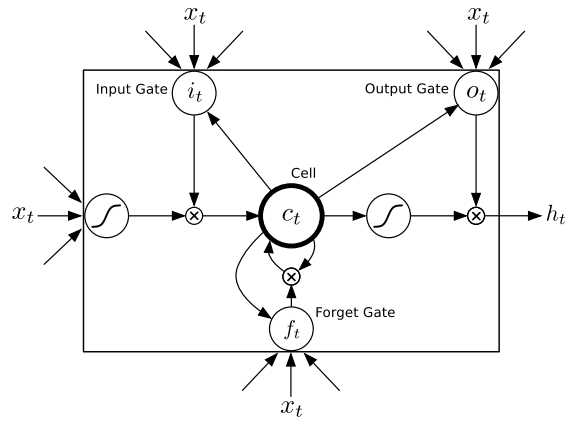
\includegraphics[width=0.7\textwidth]{img/lstm.png}
  \caption{长短时记忆模型,引自\cite{graves2013hybrid}}
  \label{fig:lstm}
\end{figure}

目前常用的递归神经网络之一是Hochreiter和Schmidhuber\cite{hochreiter1997long}提出的长短时记忆模型(Long Short-Term Memory,LSTM),其数学模型如下:

\vspace{-10mm}
\begin{equation}
\vspace{-2.5mm}
\begin{aligned}
  \label{eq:lstm}
  f_t &= \sigma_g(W_f x_t + U_f h_{t - 1} + b_f) \\
  i_t &= \sigma_g(W_i x_t + U_i h_{t - 1} + b_i) \\
  o_t &= \sigma_g(W_o x_t + U_o h_{t - 1} + b_o) \\
  c_t &= f_t \circ c_{t-1} + i_t \circ \sigma_c (W_c x_t + U_c h_{t-1} + b_c) \\
  h_t &= o_t \circ \sigma_h (c_t)
\end{aligned}
\end{equation}

其中$x_t \in \mathbb{R}^d$ 为$t$时刻的输入,$h_t$,$h_{t-1} \in \mathbb{R}^h$分别是这一时刻和上一时刻LSTM的输出(或当LSTM作为一个人工神经网络中其中一层时称为隐藏状态),$c_t \in \mathbb{R}^h$为当前时刻记忆,$i_t$,$f_t$,$o_t \in \mathbb{R}^h$分别控制了这一时刻的输入、上一时刻记忆和这一时刻的输出在这一刻起的作用,因此称为“输入门”、“遗忘门”、“输出门”的激活向量,$\sigma_g, \sigma_c, \sigma_h$为激活函数,特别地$\sigma_g$一般采用 $sigmoid$函数,$\sigma_c, \sigma_h$一般采用$tanh$函数,$W \in \mathbb{R} ^ {h \times d}, U \in \mathbb{R}^{h \times h}, b \in \mathbb{R} ^ {h}$为网络参数。和Elman网络比较可见,LSTM除了有$h_{t-1}$传递上一时刻的信息以外多了一个记忆单元$c$,具有更强的记忆功能。在LSTM的设计中包含了“输入门”、“遗忘门”、“输出门”和记忆单元,对序列数据有较强拟合能力,相对地对于小规模的序列数据容易出现过拟合。

为了解决容现出现过拟合的问题,Cho等人\cite{cho2014learning}提出了门控循环神经元(Gated Recurrent Unit, GRU)。可以认为它是LSTM的一种轻量级变型,其数学模型如下:

\vspace{-10mm}
\begin{equation}
\vspace{-2.5mm}
\begin{aligned}
  \label{eq:gru}
  z_t &= \sigma_g (W_z x_t + U_z h_{t-1} + b_z) \\
  r_t &= \sigma_g (W_r x_t + U_r h_{t-1} + g_r) \\
  h_t &= (1 - z_t) \circ h_{t-1} + z_t \circ \sigma_h (W_h x_t + U_h (r_t \circ h_{t-1}) + b_h) 
\end{aligned}
\end{equation}

可见在数学模型上GRU和LSTM非常相似,虽然GRU中省去了专门的记忆单元,但同样采用了“门”来控制当前时刻的输入和前一时刻输出的作用。GRU的模型结构要较LSTM的简单,而在同一组超参数下,GRU的模型参数要明显少于LSTM,故理论上在处理较小规模的序列数据时更有优势。

从上面的数学模型中我们不难发现,时刻$t$的输出只受时刻$t$及以前的输入影响,不过在一些场景下我们会考虑时刻$t$以后的输入是否也会与时刻$t$的输出有关。譬如在文本情感识别时,英语有一种后置定语的语法,在句子中一个单词A由出现在它后面的一组单词来修饰,那么为了正确理解在时刻$t$出现的单词A,我们就需要引入时刻$t$以后的信息。为此Schuster和Paliwal\cite{schuster1997bidirectional}提出了双向递归神经网络(Bidirectional Recurrent Neural Network,BRNN),如图\ref{fig:brnn}所示,一个双向递归神经网络包含两个RNN,对于一组序列数据,分别以其原本方向和反方向输入到两个RNN中,从而获得两个方向上与$t$时刻相关的信息。根据此思想,RNN可以替换成任何具体的递归神经网络如LSTM和GRU。

\begin{figure}[H]
  \centering
  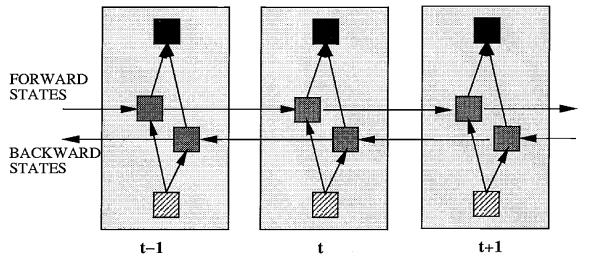
\includegraphics[width=0.7\textwidth]{img/brnn.png}
  \caption{双向递归神经网络,引自\cite{schuster1997bidirectional}}
  \label{fig:brnn}
\end{figure}

注意力机制(Attention Mechanism)受启发于人类的视觉处理机制,当人们尝试理解一个画面的内容时,他们不会马上对画面里的所有细节都进行处理,而是首先找出相关信息可能在的部位,再对该部分的内容作进一步处理。当人们对同类型画面有一定观察后,会总结出关键信息出现的模式,并在处理新的画面时优先采用这些模式来理解其中的内容。Mnih等人\cite{mnih2014recurrent}以此提出了结合递归神经网络和注意力机制来实现对手写数字的识别,不是透过预处理而是直接依赖注意力机制找出图片中数字所在的位置。其后Bahdanau等人\cite{bahdanau2014neural}同样尝试了在递归神经网络中加入注意力机制,但这次的应用场景从计算机视觉转移到了自然语言处理的机器翻译,其注意力机制的模型如下:

\vspace{-10mm}
\begin{equation}
\vspace{-2.5mm}
\begin{aligned}
  \label{eq:attention}
  e_{ij} &= a(s_{i - 1}, h_j) \\
  \alpha_{ij} &= \frac{exp(e_{ij})}{\sum\limits_{k=1}^{T_x}{exp(e_{ik})}} \\
  c_{i} &= \sum\limits_{j=1}^{T_x}{\alpha_{ij}h_j}
\end{aligned}
\end{equation}

其中$s_{i-1}$表示上一时刻($i-1$)的隐藏状态,$h_j$表示在时刻$j$的输入信息,$a$是一个计算$s_{i - 1}$和$h_j$关联性的函数,$\alpha_{ij} \in (0, 1]$表示对输出时刻$i$,给予输入时刻$j$的信息的注意力,最后根据各个时刻应该给予的注意力结合所有输入信息,得出用于时刻$i$输出的相关信息$c_{i}$。其后Vaswani等人\cite{vaswani2017attention}针对机器翻译提出了一种仅基于注意力机制搭建的人工神经网络,实验结果显示他们的模型超越了该实验数据上曾达到过最好的性能。虽然在近年不同研究\cite{luong2015effective}\cite{graves2014neural}\cite{xu2015show}中同现了各种注意力机制的变型,但这些模型可以统一描述如下:

\vspace{-10mm}
\begin{equation}
\vspace{-2.5mm}
\begin{aligned}
  \alpha_{ij} &= a(q_i, k_j) \\
  c_i &= \frac
    {\sum\limits_{j=1}^{T_x}{\alpha_{ij}v_j}}
    {\sum\limits_{j=1}^{T_x}{\alpha_{ij}}}
\end{aligned}
\end{equation}

其中$q_i$表示输出时刻$i$对应的一个请求,$k_j$和$v_j$表示输入时刻$j$的一个键值对,$a$是计算请求和键之间关联性的函数,以得出对于输出时刻$i$应给予输入时刻$j$的信息$v_j$的注意力$\alpha_{ij}$,最后以加权平均计算出输出时刻$i$相关的信息$c_i$。一些研究\cite{wang2016attention}\cite{pontiki2014semeval}则针对其中的隐藏状态$\alpha_{ij}$分析注意力机制的具体运行,并得出了和人工理解一致的结果。

\subsection{集成学习}
\label{ssec:intro_ensemble_learning}

集成学习(Ensemble Learning)的目的在于结合多个模型以达到比其中任何一个模型都要好的识别性能。集成学习方法包含了多个类别,其中常用于分类问题的是基于投票的方法,譬如多数投票(Majority Voting)、加权多数投票(Weighted Majority Vote)、加权平均概率投票(Soft Voting)。假设对于$N$分类问题,有$T$个基础模型$h^i, i = 1,2,...,T$。
对于输入数据$x$,基础模型$h^i$的输出如下:

\vspace{-10mm}
\begin{equation}
\vspace{-2.5mm}
  h^i_j(x) = 
  \begin{cases}
  1, & \mbox{若模型}h^i\mbox{将}x\mbox{识别为类别}j  \\
  0, & \mbox{其他}
  \end{cases}
\end{equation}

对于多数投票,其最终预测结果$H_M(x)$如下:

\vspace{-10mm}
\begin{equation}
\vspace{-2.5mm}
\begin{aligned}
  H_{M}(x) &= \mathop{\arg\min}_{j} \sum\limits_{i=1}^{T}h^i_j(x)
\end{aligned}
\end{equation}

在章节~\ref{sssec:traditional_ml}中提到的随机森林就是以决策树为基础模型,再采用多数投票得出最终识别结果的算法。对于加权多数投票,其最终预测结果$H_{WM}(x)$如下:

\vspace{-10mm}
\begin{equation}
\vspace{-2.5mm}
\begin{aligned}
  H_{WM}(x) &= \mathop{\arg\min}_{j} \sum\limits_{i=1}^{T}w_i h^i_j(x)
\end{aligned}
\end{equation}

其中$\sum\limits_{i=1}^{T}w_i = 1, w_i \geq 0$为每个模型的权重,相当于假设不同模型具有不同的可信度。而加权平均概率投票要求模型能给出样本在不同类别上的概率分布$p^i(x) \in [0, 1]^N$,其最终预测结果$H_S(x)$如下:

\vspace{-10mm}
\begin{equation}
\vspace{-2.5mm}
\begin{aligned}
  H_{S}(x) &= \mathop{\arg\min}_{j} \sum\limits_{i=1}^{T}w_i p^i_j(x)
\end{aligned}
\end{equation}

其中$\sum\limits_{i=1}^{T}w_i = 1, w_i \geq 0$,和加权多数投票中$w_i$的原理相同。

\section{本章小结}

在本章中,我们首先给出了面向文本的情感识别的形式化表示,描述了其中所涉及的要素并给出了对应的例子,在本论文的后续章节中,我们将利用此形式化表示套用到我们要解决的各个具体问题上,以显示各个问题之间的共性。然后我们提出了一个面向文本情感分类问题的研究框架,该研究框架的核心思想是把一个多分类问题拆解成多个子分类问题的叠加,首先对各个子分类问题进行研究,再结合各个子分类问题来解决原本的多分问题。最后我们对研究框架中涉及到的一些技术领域进行了说明,介绍了这些技术领域的目的、原理以及目前的一些主流技术,有助于读者更好的理解后续的实验以及进行拓展性的工作。












